\section{Datenbank}
\subsection{Anforderungen an die interne Datenbank}
In der internen Datenbank sollen die notwendigen Daten zum benutzerdefinierten Verarbeiten der Rezepte aus der FatSecret Datenbank abgespeichert werden. Neben den Userdaten und den Userpräferenzen werden Rezept-IDs, Allergene, Unverträglichkeiten und die Produkte für die Einkaufsliste gespeichert. Die FatSecret Datenbank stellt Rezepte mit Kochanleitungen und Nährstoffangaben zu Verfügung und ordnet diese abhängig von ihren Eigenschaften in unterschiedliche Kategorien ein. So befinden sich zum Beispiel alle Rezepte mit einem hohen Proteinanteil unter der Kategorie „high-protein“ und können somit schnell herausgefiltert werden. Es gibt dennoch notwendige Informationen, die FatSecret nicht beinhaltet. Die Allergene. Dafür sollen alle Allergene recherchiert werden und in die interne Datenbank geladen werden. Später können sie verwendet werden um mit dem Algorithmus die Rezepte durchzusuchen und die Speisen, auf die der User allergisch ist, weg zu geben.

Für die interne Datenbank sind folgende Anforderungen gesetzt: \linebreak
Die logische Struktur der FatSecret Datenbank soll rekonstruiert und in die interne Datenbank mit übernommen werden. Abgespeichert werden die IDs der Rezepte und die Userdaten mit ihren Präferenzen. Diese sollen über einen Plan verbunden werden, der je nach Userangaben wochentagabhängig anpassbar ist. Die unterschiedlichen Allergene sollen in einer eigenen Tabelle stehen und den Usern zuordenbar sein. Zusätzlich sollen die Produkte aus der Einkaufsliste in der Datenbank vorkommen. Da nicht alle Daten aus einer anderen Datenbank kommen und schnell weiter verarbeitet werden, muss Wert darauf gelegt werden, dass die Verbindung verzugsfrei funktioniert. Mehrere User sollen gleichzeitig den Plan generieren lassen können. Dabei werden sehr viele Zugriffe sowohl auf die FatSecret API als auch auf die interne Datenbank gemacht.

\subsection{Relationale und nicht-relationale Datenbanken}
\subsubsection{Relationale Datenbanken}
In einer relationalen Datenbank werden Daten in miteinander über ein Fremdschlüssel verbundenen Tabellen gespeichert. Jede Tabelle besteht aus Spalten (genannt Attribute) und Zeilen (Datensätze). Jede Spalte hat einen eigenen Informationstyp.  Einige Attribute sind Informationen zu der Tabelle. Andere enthalten Verweise, Fremdschlüssel, auf Primärschlüssel, einem logischen oder künstlich festgelegten Indikator, anderer Tabellen. Beziehungen sind das Hauptmerkmal dieses Modells. 

Tabellen in relationalen Datenbanken müssen einigen Kriterien entsprechen, sie müssen „normalisiert“ werden. Mit der Normalisierung können Anomalien und Redundanzen vermieden und Konsistenz sichergestellt werden.

\begin{description}
\item 1NF \\
Die erste Normalform besteht, wenn alle Attribute atomar sind. Das bedeutet nicht mehr weiter trennbar. Zusätzlich dürfen Datensätze nicht mehrmals vorkommen. Dafür werden zusammenhängende Daten wie zum Beispiel Adresse in Ort, Stadt und PLZ getrennt. Dieser Schritt macht es möglich die einzelnen Adressteile anzusprechen.
\item 2NF \\
Eine Tabelle entspricht dann der zweiten Normalform, wenn sie der 1NF entspricht und jedes Nichtschlüsselattribut von dem gesamten Schlüsselattribut abhängt. Das stellt sicher, dass alle Informationen einer Tabelle logisch zusammenhängen. Besitzt eine Tabelle in der ersten Normalform nur ein Primärschlüssel, so entspricht die Tabelle auch gleichzeitig der zweiten Normalform. \linebreak  Als Beispiel kann man sich eine Restaurantrechnung vorstellen. Diese hat als Primärschlüssel die Rechnungsnummer und die Kundennummer. Zusätzlich stehen aber in der Tabelle der Preis und die Personendaten des Kunden. Diese hängen nicht direkt mit beiden Primärschlüsseln zusammen und können somit in externe Tabellen ausgelagert werden.
\item 3NF \\
Bei der dritten Normalform muss die Tabelle der 2NF entsprechen und kein Nichtschlüsselattribut darf von einem anderen Nichtschlüsselattribut transitiv abhängen. Wenn also das Attribut B von A abhängt und das Attribut C von B, muss C in eine externe Tabelle ausgelagert werden, da C nur indirekt von A abhängt. Kurzgefasst bedeutet es, dass die Nichtschlüsselattribute nur direkt von einem Schlüsselattributen abhängen dürfen. Hat eine Tabelle mit Kundendaten auch die Postleitzahl drinnen, so hängt die Postleitzahl von der Adresse, aber nicht direkt von dem Kunden ab. So kann man die Postleitzahl auslagern und über eine Zwischentabelle mit dem Kunden verbinden.
\end{description}

Relationale Datenbanken werden mit der strukturierten Abfragesprache SQL „Structured Query Language“ erstellt, befüllt, gelöscht und bearbeitet. In den 70er Jahren unter der Bezeichnung SEQUEL „Structured English Query Language“ veröffentlich ist SQL mittlerweile der Standard für die Datenbankinteroperabilität, also der Besonderheit Systeme einwandfrei miteinander zusammenzuführen. SQL ist die Grundlage für die aktuellen Datenbankanwendungen, unter anderem Oracle.

\paragraph{Datenbankentwicklung mit MySQL\cite{MySQLigegenPDO}} 

Die Beliebtheit von MySQL stieg schon in den 90er Jahren wegen des freien Sourcecodes. MySQL wird im Allgemeinen mit der Programmiersprache PHP und dem Apache Web Server in Linux-Distributionen verwendet, was zur Abkürzung LAMP (Linux, Apache, MySQL, PHP) für das Open Source-Programmpaket führte. Bei Windows kennt man es unter XAMPP (cross-platform, Apache, MySQL, PHP, Perl).
In der Entwicklung von MySQL ermöglicht unter anderem MySQLi die Verbindung zwischen PHP und der MySQL-Datenbank. MySQLi (improved) ist eine aktualisierte Version des PHP-MySQL-Treibers. Es unterstütz objektorientierte und prozedurale Programmierung. Es beinhaltet Prepared Statements, die Angriffe durch SQL-Injections verhindern. Mit den SQL-Injections können von Hackern Befehle eingeschleust werden, die etwas an der Datenbank verändern können. \linebreak Sowie MySQLi, stellt PDO „PHP Data Objects“ auch eine Schnittstelle zwischen PHP und Datenbanken zu Verfügung. Es ist mit 11 anderen Datenbanksystemen zusätzlich zu MySQL kompatibel und unterstützt ebenso wie MySQLi die Prepared Statements. 
2010 wurde MySQL von Oracle übernommen und erlangt seit dem immer mehr Kritik. \cite{KritikanderMySQLDatenbank} Der Grund dafür sind die eingeschränkten Möglichkeiten der freien Version im Gegensatz zu denen der kommerziellen Version. Viele neue Funktionen werden nur mehr von der kostenpflichtigen Version unterstützt oder erst viel später in die neuen Updates eingebunden. Daraus folgt die Entscheidung auf das zwar erlernte, aber im späteren Verlauf kostenpflichtige MySQL zu verzichten.

\paragraph{Datenbankentwicklung mit Oracle}
Die Oracle-Datenbank ist ein relationales Datenbankverwaltungssystem von der Oracle Corporation. Der Zugriff erfolgt über SQL. Die Erweiterung von SQL für die Arbeit mit Oracle heißt PL/SQL „Procedural Language“, sie verknüpft die prozedurale Programmiersprache mit dem gewohnten SQL. Es wurde von der Oracle Corporation entwickelt, um die SQL-Funktionen zu erweitern. Auf Grund der kostenpflichtigen Lizenzen ist Oracle für die Anwendung nicht geeignet.

\subsubsection{Nicht-relationale Datenbanken}
\paragraph{Nicht-relationale Datenbanken mit NoSQL }
NoSQL \cite{NoSQL} „Not only SQL“ Datenbanken unterscheiden sich stark von dem relationalen Modell. SQL folgt einem strikten Schema und hat eine genau definierte Struktur. Die Datentypen und Integritätsbedingungen sind genau vordefiniert und es gibt wenig Spielraum. Bei NoSQL beinhalten die Datensätze gleich ihre Beschreibung und es ist kein einheitliches Abfrageformat definiert. Es ist vergleichbar mit den JSON und XML Formaten, bei denen die einzelnen Felder einen Namen haben, der sie definiert. Nicht-relationale Datenbanksysteme erstellen eine Struktur im laufenden Betrieb, erlauben jeden Datentyp und speichern Objekte, Listen, Wertepaare und Dokumente. NoSQL erleichtert die Speicherung und den Zugriff auf Daten. Das am weitesten verbreitete  NoSQL Datenbanksystem ist MongoDB. 
\subsubsection{Entscheidung}
Wenn es um Datenintegrität geht, nehmen SQL-Datenbank-Transaktionen immer noch eine führende Position ein. Die Art und Weise wie eine NoSQL Datenbank programmiert wird muss von Anfang an erlernt und angeeignet werden. Auf Grund der im oberen Absatz genannten Argumente und dem Zeitvorteil, der durch das schon Erlernte während dem Unterricht entsteht, fällt die Entscheidung auf eine relationale Datenbank. Zusätzlich erfordert die interne Datenbank eine festgelegte Struktur und definierte Datentypen damit die Verbindungen zwischen dem Plan, den Allergenen und den Userpräferenzen genau in den Algorithmus eingebaut werden können.

\subsection{Open Source Datenbanken}
Von den relationalen Open Source Systemen stehen folgende zur Verfügung: 

\subsubsection{MariaDB \cite{MariaDBDefinition}} 
MariaDB wurde vom selben Entwickler geschrieben wie MySQL. Es ist eine Abspaltung von MySQL und ihr Hauptziel besteht darin, weiterhin ein Open Source Datenverwaltungsprogramm anzubieten. Gleichzeitig soll es erhebliche Verbesserungen des Codes mit sich bringen. Wegen der Ähnlichkeit kann Zeit für das Erlernen des Codes gespart werden. MariaDB wird öfters auf Grund der häufigen Sicherheitupdates MySQL vorgezogen. MariaDB wird völlig offen entwickelt, alle Lösungen und neuen Ideen zur Entwicklung können im E-Mail-Newsletter sowie im Fehlermeldungssystem frei diskutiert werden. 

\subsubsection{PostgreSQL \cite{PostgreSQLAnwendungsfall}}
PostgreSQL ist ein leistungsfähiges Open Source System. Ebenso wie andere relationale Datenbanksysteme unterstütz es das Transaktionskonzept von SQL, das ACID-Konzept (Atomicity, Consistency, Isolation, Durability). Das beschreibt Kriterien, die von SQL-Datenbanken verwendet werden, um sicherzustellen, dass Datenbankänderungen konsistent, sicher und dauerhaft gespeichert werden.

Basierend auf der leistungsstarken Technologie bewältigt PostgreSQL die gleichzeitige Bearbeitung mehrerer Aufgaben. Die Datenbank ist weit skalierbar, flexibel und kann in sehr vielen Programmiersprachen verwendet werden. Nach einer richtigen Einrichtung der Programmierumgebung verläuft die Verwaltung der Datenbanken sehr schnell. Ein weiteres Feature ist die Unterstützung von JSON Format, was eine schemalose Speicherung ermöglicht. Dies kann nützlich sein, wenn die Datenstruktur ein gewisses Maß an Flexibilität erfordert: Wenn sich zum Beispiel die Struktur während des Entwicklungsprozesses noch ändert und unbekannt ist, welche Felder das Datenobjekt enthalten wird. 

Zusätzlich ist der Entwicklersupport auf hohem Level und die Community groß. Bei PostgreSQL wird viel Wert auf die Sicherheit und Stabilität der Daten gelegt, ebenso wie auf Integrationsmöglichkeiten und das Verwalten und Erweitern komplexer Prozesse. 

\subsubsection{SQLite \cite{SQLiteDefinition}}
SQLite ist in Form einer Bibliothek in die Anwendung eingebettet und funktioniert ganz ohne einem eigenen Server. Die meisten SQL-Datenbankmodule werden als separater Serverprozess erstellt. Programme, die auf die Datenbank zugreifen möchten, kommunizieren mit dem Server über Prozessinteraktionen (normalerweise TCP/IP), um Anforderungen an den Server zu senden und die Ergebnisse zurückzuholen. SQLite arbeitet anders. In SQLite liest und schreibt ein Prozess, der auf eine Datenbank zugreifen möchte, direkt aus den Datenbankdateien auf der Festplatte. Dadurch werden die Vermittlungsprozesse des Servers nicht benötigt. Die ganze Verwaltung funktioniert mit PHP. All das verbessert die Geschwindigkeit und Leistung der Vorgänge. Auf Grund des geringen Speicherbedarfs wird SQLite oft bei embedded Systemen angewendet, zum Beispiel bei Handy Applikationen.

Die Implementierung verläuft sehr schnell, die Datenbank ist auf Grund ihrer Bau- und -Funktionsart für das schnelle Anlegen kleiner Projekte, auch Prototypen ausgelegt. Durch das kleine Format sind die Fähigkeiten von SQLite beschränkter als die von MySQL\cite{SQLiteLimitierungen}. Befinden sich die Daten auf einer anderen Datenbank, auf die über das Netz zugegriffen werden muss, so ist SQLite nicht die optimalste Lösung. Die Engine-zur-Disk Verbindung müsste mit einer höheren Bandbreite über das Netzwerk laufen. Ebenso wird es nicht empfohlen, wenn mehrere User gleichzeitig an der Datenbank Änderungen vornehmen. SQLite unterstützt nicht mehr als eine Userinteraktion mit einer Tabelle zum selben Zeitpunkt. Eine Datenbank-Engine, die einen Server verwendet, kann zusätzlich einen besseren Schutz vor Fehlern in der Clientanwendung bieten als SQLite: Ein parasitärer Zeiger im Client kann nämlich den Speicher auf dem Server nicht zerstören.

\subsubsection{Auswahl der passenden Datenbank} 
Laut dem Ranking von DB-Engines \cite{DBRanking}, von Februar 2019, steht PostgreSQL auf dem 4 Platz, SQLite auf 10 und MariaDB auf Platz 12. Die Plätze darüber besetzen kostenpflichtige Datenbankentwicklungtools. Die Entwicklung von PostgreSQL begann in den 1980ern und gewinnt seit dem immer mehr Unterstützung von der Entwicklercommunity. 

Eines der Ziele der Diplomarbeit ist es neue Techniken und Programme innerhalb der Entwicklungszeit auszuprobieren und sich diese anzueignen. Aus diesem Grund fällt MariaDB weg, da im Unterricht in MySQL entwickelt wurde und diese Umgebungen sehr ähnlich sind. SQLite ist zwar schnell und leicht zu implementieren, die Größenlimitierungen reichen für das Projekt aus und dennoch kommen die Daten aus einer externen Datenbank, die über das Netzwerk zu erreichen ist, dadurch könnten hohe Wartezeiten entstehen. Daraus folgt die Entscheidung PostgreSQL als Verwaltungsprogramm für die projektinterne Datenbank zu wählen. Es läuft auf einem Server, unterstützt viele Userabfragen gleichzeitig, ist flexibel und auf alle Projektstrukturen anpassbar. 

\subsection{Erstellen und Verwalten der Datenbankstruktur}

\begin{figure}[hb]
\centering
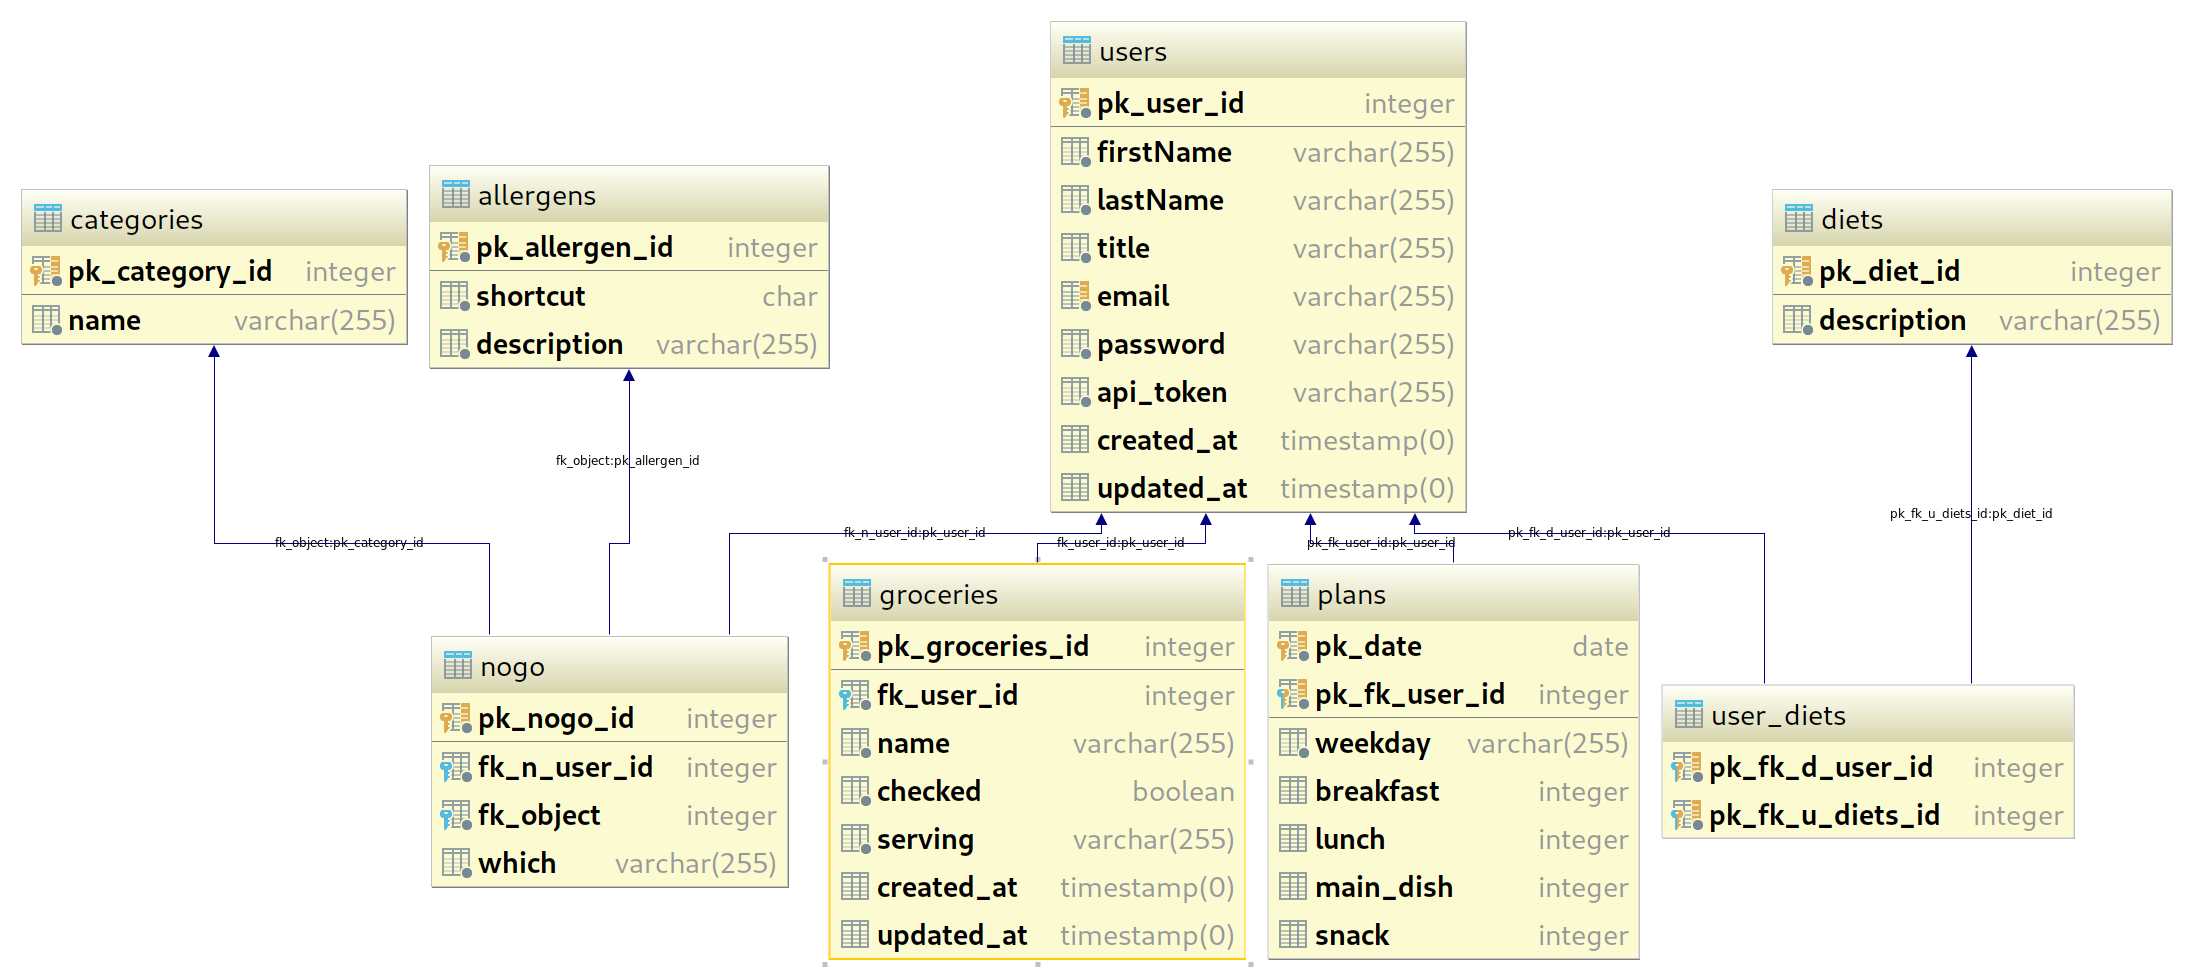
\includegraphics{threesixfive.png}
\caption{ER-Modell}
\end{figure}

\paragraph{Der Plan}
Der Plan wird nach Tagen mit Daten aufgeteilt und einer Person zugeteilt. Pro Tag wird ein Plan erstellt, der pro Mahlzeit (Frühstück, Mittagessen, Hauptspeise und Snack) eine Rezept-IDs aus der FatSecret Datenbank enthält. Mit Hauptspeise ist das Abendessen gemeint, die Definition kommt aus der FatSecret Datenbank.
Sollte in dem Anmeldungsformular festgelegt werden, dass Montags keine Frühstücke gibt, so werden alle Frühstückseinträge mit dem Backendalgorithmus auf NULL gesetzt. Das weekday-Feld erleichtert die Arbeit für das Algorithmus, so muss nicht zusätzlich bei jeder Abfrage aus dem Datum der Wochentag ermittelt werden. 

\paragraph{No-Gos}
Wenn ein User eine Allergie (allergens) oder ein Produkt aus der Liste der typischen Unverträglichkeiten (categories, eine Definition aus der FatSecret Datenbank) angibt, so wird es in der „nogo“-Tabelle eingetragen. Das Feld "which" legt fest ob es eine Allergie oder Unverträglichkeit ist, so kann man die zwei Tabellen leichter in dem Algorithmus von einander unterscheiden. Ist zum Beispiel ein User auf Fisch allergisch, so füllt er das in dem Registrierungsformular aus und es wird ein Eintrag in die „nogo“-Tabelle gemacht. In das Feld „fk\_object“  wird die Allergen-ID von Fisch geschrieben, das Feld "which" mit einem "a" befüllt und beim Algorithmus darauf geachtet, dass nur Rezepte vorgeschlagen werden, die kein Fisch enthalten. Die Intoleranzen sind eine festgelegte Liste an Produkten, die oft nicht gerne gegessen werden. Darunter fallen Meeresfrüchte, Soja, Nüsse, Schweinefleisch, Rindfleisch und vieles andere. Gibt der User dies in dem Formular an, so gibt es ebenso einen Eintrag in der „nogo“-Tabelle. Somit hat ein User mehrere „nogo“-Einträge, die bei dem Algorithmus direkt berücksichtigt werden.
\paragraph{Groceries}
Die Einkaufsliste speichert alle notwendigen Produkte für die kommende Woche. Das „checked“-Statusfeld wird dann auf true gesetzt, wenn das Produkt in der Liste abgehackt, also gekauft, wurde. Die Felder "created\_at" und "updated\_at" sind notwendig um festzustellen seit wann das Produkt in der Liste ist und ob es seit einer Woche abgehackelt ist, dann kann das Produkt aus der Liste entfernt werden.
\paragraph{Diets}
Beim Generieren des Plans werden Diäten, falls eine Diät ausgewählt ist, die in der „diet“-Tabelle stehen, miteinberechnet. Verfügbare Diäten sind „Milchfrei“, „Glutenfrei“, „High Protein“, „Kalorienarm“ und „Low Carb“. Je nach der ausgewählten Diät werden bestimmte, in der FatSecret API implementierte, Tags zur Abfrage hinzugefügt, um somit die Rezepte zu filtern. Zum Beispiel werden bei „High“-Protein automatisch Rezepte genommen, die den „high-protein“-Tag haben und somit einen hohen Anteil an Protein besitzen.

\paragraph{Users}
Die User-Tabelle speichert die typischen Userdaten, wie Name, Nachname, Titel sowie zur Anmeldung notwendige E-Mail-Adresse und das verschlüsselte Passwort. Die Fehlder "created\_at" und "updated\_at" werden für Operationen im Algorithmus gebraucht.

\subsubsection{Datenbankverwaltungstools}
Der erste Schritt von der Einrichtung einer PostgreSQL Entwicklungsumgebung ist den Installer herunterzuladen. Der Installer beinhaltet die PostgreSQL Engine, das Paketverwaltungsprogramm StackBuilder und ein grafisches User Interface für die Datenbankverwaltung pgAdmin. 

Die Datenbank soll während ihrer Entwicklung nur lokal laufen. Aus diesem Grund gibt man als Speicherort den C:/xampp Ordner an. XAMPP ist ein von Apache entwickeltes Open Source-Paket für plattformübergreifende Webserverlösungen, das hauptsächlich aus dem Apache HTTP Server, der MariaDB-Datenbank und Interpreter für die Programmiersprachen PHP und Perl besteht. Es ist erweiterbar und PostgreSQL lässt sich leicht einbinden, in dem man die heruntergeladenen Ordner unter C:/xampp/pgsql hinterlegt. Zum Starten und Stoppen des PostgreSQL Servers muss man unter Windows 10 die services.msc (Windows Dienste) öffnen und mit einem Rechtsklick auf PostgreSQL 11.xx (Versionsnummer) starten, beenden oder anhalten wählen.


Mit PgAdmin lässt sich die Datenbank ganz leicht generieren und die Daten verwalten. Dennoch kann man zusätzlich phpPgAdmin installieren um die Administration der Datenbank zu erleichtern.\cite{PostgreSQLVerwaltungstools} Dazu muss man die Installationsdateien in einem neuen Ordner C:/XAMPP/phpPgAdmin hinterlegen und die Inhalte der Dateien C:/XAMPP/phpPgAdmin/conf/config.inc.php, C:/XAMPP/php/php.ini und C:/XAMPP/apache/conf/extra/http-xampp.conf ändern. In der ersten Datei muss \codeword{\$conf[‚extra\_login\_security‘]} auf „false“ gesetzt werden und in der zweiten muss die Zeile \codeword{;extension=php\_pgsql.dll} aktiviert werden in dem man den Kommentar „;“ davor entfernt. Die http-xampp.conf Datei muss um folgende Zeilen erweitert werden: 

\begin{verbatim}
Alias phppgadmin „C:/XAMPP/phppgadmin/“
<Directory „C:/XAMPP/phppgadmin“>
Options Indexes FollowSymLinks MultiViews
AllowOverride all
Require local
Order Deny,Allow
Allow from all
</Directory>
 \end{verbatim}

Jetzt kann man nach dem Starten des Apache Servers über den Browser unter localhost/phppgadmin auf PhpPgAdmin zugreifen.
